
\chapter{Evaluation}\label{chapter:evaluation}

In this chapter, the presented approach is evaluated regarding performance, safety properties, and general feasibility. For this, a number of tests were conducted which are described in the following.

\section{Test Setup}

The network topology used in the tests is depicted in \autoref{fig:network-topology}. In the local test environment ("on-premise") there is a cluster of three ARM-based SOCs\footnote{System on a Chip} (Raspberry Pi 3) which are connected over a Gigabit LAN switch (left-hand side). The three nodes represent on-board computing devices in a hypothetical vehicle. Connected to the LAN is also a workstation which fulfills the sole purpose of orchestrating the tests, \ie , it is not directly involved in the test execution per se. The local test environment is connected to the remote data center over the open Internet via 100 Mb/s connection.

\begin{figure}[htpb]
  \centering
  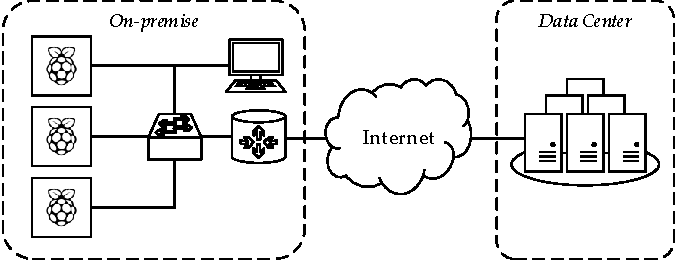
\includegraphics[width=\textwidth]{figures/network-setup}
  \caption[Network topology]{The network topology in the test setup}\label{fig:network-topology}
\end{figure}
%
Representative of the "cloud" in the tests is a single root server supplied by the IaaS provider \emph{DigitalOcean}\footnote{\url{www.digitalocean.com}} (right-hand side in \autoref{fig:network-topology}). To ensure realistic latency values, a server location was chosen that was in the vicinity of the test setup -- but not too close. Considering its vicinity to Munich, Frankfurt (Main) was a suitable choice. The two cities are about 300 km away from each other (as the crow flies).

The detailed specifications of the involved computing nodes are given in \autoref{tab:test-specs}
%
\begin{table}[htpb]
  \caption[Test environment specifications]{Test environment specifications}\label{tab:test-specs}
  \centering
  \begin{tabular}{p{0.235\textwidth} | p{0.335\textwidth}  p{0.335\textwidth}}
    \toprule
       & \textbf{On-premise} & \textbf{Remote} \\
    \midrule
    	Description & Raspberry Pi 3 Model B  & DigitalOcean 1 GB Droplet\\
    	Number of nodes & 3  & 1\\
    	\midrule
    	Operating system & Raspbian GNU/Linux 9.3  & Ubuntu 16.04.3 LTS\\
    	Kernel & 4.9.59-v7+ w/ real-time patch \emph{PREEMPT\_RT} 4.4.9-rt17 & 4.4.0-112-generic \\
      CPU & ARMv7 rev 5  Quad Core (1.2 GHz) & Intel(R) Xeon(R) E5-2650 v4 Single Core (2.20GHz) x86\_64 \\
      Memory (RAM) & 1 GB & 1 GB  \\
      Network connection  & 100 Mb/s & 40 Gb/s\\
      \midrule
      DDS & \multicolumn{2}{c}{OpenDDS 3.12.1}\\
      Docker  & \multicolumn{2}{c}{17.11.6-ce}\\
      Weave Net & \multicolumn{2}{c}{2.2.0}\\
    \bottomrule
  \end{tabular}
\end{table}
%
%
%
%
%
%
%
%
%
%

\section{Latency Benchmark}

\paragraph{Motivation.} An essential non-functional requirement for computer networks is responsiveness. An often-used metric for responsiveness is latency which is measured by the time a packet needs to be sent from one peer to another and back again (round-trip). 

To evaluate the aptitude of the proposed approach it is essential to consider the latency overhead that overlay networks induce. Since the approach is intended to work over the Internet, and public networks are inherently insecure, encryption is vital. Thus, in addition to the overhead induced by the overlay network itself, the overhead caused by encryption is also of interest. Hence, tests are needed measuring latency not only of \emph{plain} overlay networks but also of \emph{encrypted} overlay networks.


\paragraph{Methodology.} 

\begin{figure}[htpb]
  \centering
  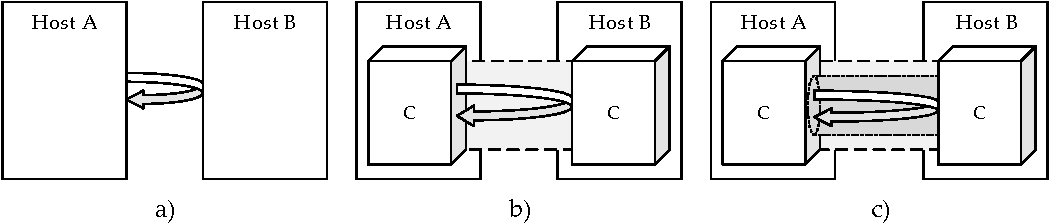
\includegraphics[width=\textwidth]{figures/ping-test}
  \caption[Latency experiment setup]{Latency experiment setup. a) \experim{Plain}: two hosts connected without containerization. b) \experim{Weave}: two containers connected via Weave Net. c) \experim{Encrypted}: two containers connected via encrypted Weave Net channel.}\label{fig:latency-setup}
\end{figure}

In this test, latency was measured between two hosts connected over the Internet, both with and without container networking. A constant stream of ping messages was sent from one of the Raspberry Pis to the remote host. The tests were repeated with multiple payload sizes to factor in the influence of message size on round trip times. The Linux tool \emph{ping}, which pings hosts via ICMP Echo Requests and Replies, was employed for the measurements. 

Three experiments were conducted, comparing the average latencies of plain, host-to-host communication ("\experim{Plain}"), via Weave Net ("\experim{Weave}") and when employing encryption over Weave Net ("\experim{Encrypted}") (\cf \autoref{fig:latency-setup}). \experim{Plain} was used as baseline on the basis of which the two consecutive experiments were evaluated. For each experiment and message size, 300 ping messages were sent. The sending peer would wait for the response of the previous message before sending another request. Thus, only one transaction was in flight at a time.


\paragraph{Results.} 

\autoref{fig:latency-relative} depicts the absolute and relative latency measures of the tested network modes. Values represent the average round trip time of the 300 sent messages. The relative overhead is calculated from ratio of \experim{Weave} and \experim{Encrypted} when compared to \experim{Plain}, respectively. The results show that the network latency induced by Weave Net (without encryption) is hardly measurable and therefore negligible. Message size has no influence whatsoever in this comparison. 


\begin{figure}[htpb]
  \centering
  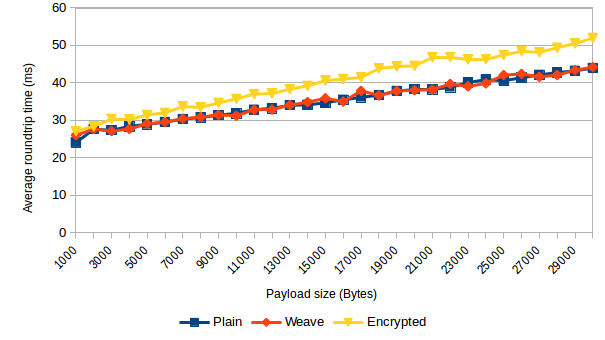
\includegraphics[width=0.49\textwidth]{figures/latency-absolute}
  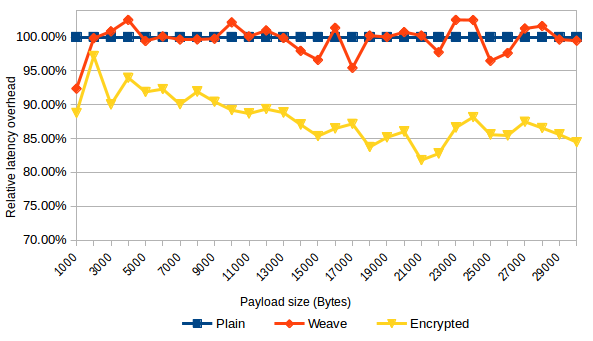
\includegraphics[width=0.49\textwidth]{figures/latency-relative}
  \caption[Latency overhead]{Absolute (a) and relative (b) latency overhead of \experim{Weave} and \experim{Encrypted} over \experim{Plain}}\label{fig:latency-relative}
\end{figure}

However, the tests revealed that encryption over Weave Net (\experim{Encrypted}) adds quite a hefty base overhead which further increases with message size. For the smallest messages the overhead started at roughly 5\% and went up to over 15\% for messages with 30 KB payload. The encryption overhead may therefore be considered significant.

\begin{figure}[htpb]
  \centering
  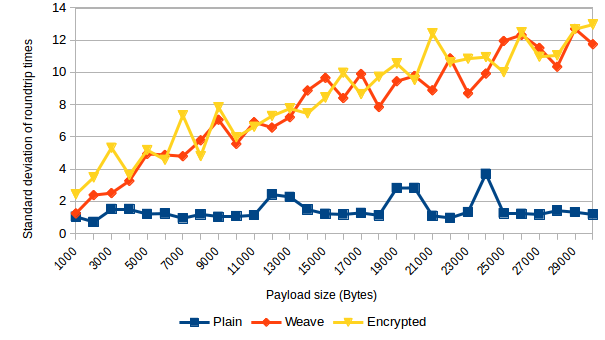
\includegraphics[width=0.8\textwidth]{figures/latency-stdev}
  \caption[Latency deviation]{Standard deviation of latencies in the scenarios \experim{Plain}, \experim{Weave} and \experim{Encrypted}}\label{fig:latency-stdev}
\end{figure}

Another insight worth mentioning is that Weave Net added significant deviations in latency that increased with message size (\cf \autoref{fig:latency-stdev}). Whether the connection was encrypted or not made little difference. Real-time systems need to behave in a predictable manner. The experiments show that routing traffic through overlay networks had a substantial, negative impact on predictability of the communication channel. From the viewpoint of real-time systems this is a serious drawback of the presented approach. 



%
%
%
%
%
%
%
%
%
%

\section{DDS Latency Benchmark}

\paragraph{Motivation.} Motivation asldfkj safdl jdsafljdsa flsa dflkdsa jfldsakjf saldkjf saldfj salkdfj ldsafkj dsalkfj dsalkfj sadlkfj dsaflkjdsa flkdsaj flkdsa jfdsalfk 

\paragraph{Methodology.} Methodology

\paragraph{Results.} Results

%
%
%
%
%
%
%
%
%
%

\section{Throughput Benchmark}

\paragraph{Motivation.} Motivation

\paragraph{Methodology.} Methodology

\paragraph{Results.} Results

%
%
%
%
%
%
%
%
%
%

\section{Failover Test}

\paragraph{Motivation.} The presented approach offers entirely new opportunities for innovation. For instance, consider the following scenario: A service running on an on-board computer within a vehicle suddenly fails, \eg\ due to a hardware defect. As a reaction, a fallback service needs to take over. Consider now that the fallback service is not running on another on-board computer but within the cloud. Enabled by DDS' failover qualities, the presented approach allows a quick switch to the remote backup service. An interesting question is how long the whole failover process, \ie\ switching to a backup service in case of failure, takes in a cloud scenario.

\paragraph{Background.} The failover mechanism is driven by DDS. When DDS "observes" that a given service is unresponsive it automatically instructs another service to take over, provided that one exists. This mechanism is realized via the QoS policies \ownership , \ostrength\ and \liveliness\ . 

By assigning a topic the \ownership\ value "\qos{exclusive}" one can specify that only a single data writer may write to that topic at any given time. Which data writer is given that prerogative is determined by the data writer's \ostrength\ value. The data writer that possesses the higher value is eligible to write to the topic.

\liveliness\ is used to determine whether a data writer or data reader is "alive", \ie , responsive. For data writers, it is sufficient that it writes within a specified time interval in order to be considered "alive". For data readers, on the other hand, there are several ways in which it can signal liveliness. One way is to send continuous "heartbeat" messages.

\ownership\ can be combined with \liveliness\ to realize a failover mechanism.
\todo[inline]{how exactly?}

In the following an example is given describing how this failover meachnism was leveraged in a cloud scenario.


\newcommand{\proda}{\texttt{S\textsubscript{main}}}
\newcommand{\prodb}{\texttt{S\textsubscript{backup}}}
\newcommand{\cons}{\texttt{S\textsubscript{consume}}}

\paragraph{Methodology.} To test the performance of DDS's failover qualities an experiment was designed to replicate a scenario in which a service fails so that another, remote service takes over operation. There are three services: two services which continuously produce data (\proda , \prodb) and one which consumes the data (\cons). \proda\ has precedence over \prodb\ (\ie\ higher \ownership\ value) and is therefore the "main supplier", while \prodb\ is considered the "backup supplier". 

In the process of sending data, a failure of \proda\ is simulated by abruptly shutting down the application process. Once that happens, a procedure in \cons\ is triggered to determine the time span between the reception of the last message sent by \proda\ and the first message by \prodb . The resulting time is the effective gap between the reception of two messages which includes
\begin{itemize}
  \item the time DDS needs to detect \proda 's change of liveliness and to propagate the change in the system
  \item the time it takes \prodb\ to take over
  \item the transmission time of \prodb 's first message to \cons
\end{itemize} 

\proda\ and \cons\ are deployed as individual applications on two of the Raspberry Pis. \prodb\ is deployed on the remote host. All communication goes through an encrypted Weave network spanning over the LAN and the cloud.

\todo[inline]{which QoS settings were used? how many test runs were conducted?}



\paragraph{Results.} Results

%
%
%
%
%
%
%
%
%
%

\section{Case Study}

\paragraph{Motivation.} Motivation

%
%
%
%
%
%
%
%
%
%


\section{Limitations}

The benchmarks in the previous sections demonstrated that the approach to cloud connectivity presented in this thesis is fully functional. However, there are some limitation that need to be addressed.

Firstly, Weave Net is not designed to be used in safety critical systems. On their website, Weaveworks make no statement about any certification efforts that make the software suitable for the use in safety-critical systems. Thus, for the time being, the given approach may only find applicability for non-safety critical functions, \eg in the context infotainment systems. However, it may be added that Weave Net is Open Source, and as such, all underlying technologies and concepts are disclosed. Thus, it is feasible to implement a thoroughly verified version of Wave Net tailored towards safety-critical systems.

In the context of vehicles, safety is inherently connected to the software system's security. Hence, proper methods are required to ensure the system's authenticity, confidentiality, integrity and privacy properties. The presented approach was not tested regarding these attributes. A rigor security analysis is needed to be able to make a well-founded statement about its aptitude.

It may also be noted that the Docker images presented in this thesis are by no means production ready. Although there was an effort to minimize the size of the images, in real scenarios, images would be shaved down to the bare minimum, both in terms of size and capabilities. Utilities such as compilers, build tools and generally everything which is not a prerequisite to execute a given service would be removed. The images used in this thesis serve the purpose of demonstration and thus, such measures were not taken to ensure a rapid progression of this work. More time would be needed to optimize the images for production use.


%
%
%
%
%
%
%
%
%
%
%
%
%
%
%
%
%
%
%
%
%
%
%
%
%
%
%
%
%
%
%
%